\documentclass[journal,12pt,twocolumn]{IEEEtran}
%
\usepackage{setspace}
\usepackage{gensymb}
\usepackage{xcolor}
\usepackage{caption}
%\usepackage{subcaption}
%\doublespacing
\singlespacing

%\usepackage{graphicx}
%\usepackage{amssymb}
%\usepackage{relsize}
\usepackage[cmex10]{amsmath}
\usepackage{mathtools}
%\usepackage{amsthm}
%\interdisplaylinepenalty=2500
%\savesymbol{iint}
%\usepackage{txfonts}
%\restoresymbol{TXF}{iint}
%\usepackage{wasysym}
\usepackage{amsthm}
\usepackage{mathrsfs}
\usepackage{txfonts}
\usepackage{stfloats}
\usepackage{cite}
\usepackage{cases}
\usepackage{subfig}
%       \usepackage[latin1]{inputenc}
       \usepackage{fullpage}
       \usepackage{color}
       \usepackage{array}
       \usepackage{calc}
       \usepackage{multirow}
       \usepackage{hhline}
       \usepackage{ifthen}


%\usepackage{xtab}
\usepackage{longtable}
\usepackage{multirow}
%\usepackage{algorithm}
%\usepackage{algpseudocode}
\usepackage{enumitem}
\usepackage{mathtools}
\usepackage{iithtlc}
%\usepackage[framemethod=tikz]{mdframed}
\usepackage{listings}
\usepackage{tikz}

%\usepackage{stmaryrd}


%\usepackage{wasysym}
%\newcounter{MYtempeqncnt}
\DeclareMathOperator*{\Res}{Res}
%\renewcommand{\baselinestretch}{2}
\renewcommand\thesection{\arabic{section}}
\renewcommand\thesubsection{\thesection.\arabic{subsection}}
\renewcommand\thesubsubsection{\thesubsection.\arabic{subsubsection}}

\renewcommand\thesectiondis{\arabic{section}}
\renewcommand\thesubsectiondis{\thesectiondis.\arabic{subsection}}
\renewcommand\thesubsubsectiondis{\thesubsectiondis.\arabic{subsubsection}}

% correct bad hyphenation here
\hyphenation{op-tical net-works semi-conduc-tor}
\def\inputGnumericTable{}                                 %%
\lstset{
%language=Python,
frame=single, 
breaklines=true
}

%\lstset{
	%%basicstyle=\small\ttfamily\bfseries,
	%%numberstyle=\small\ttfamily,
	%language=Octave,
	%backgroundcolor=\color{white},
	%%frame=single,
	%%keywordstyle=\bfseries,
	%%breaklines=true,
	%%showstringspaces=false,
	%%xleftmargin=-10mm,
	%%aboveskip=-1mm,
	%%belowskip=0mm
%}

%\surroundwithmdframed[width=\columnwidth]{lstlisting}


\begin{document}
%

\theoremstyle{definition}
\newtheorem{theorem}{Theorem}[section]
\newtheorem{problem}{Problem}
\newtheorem{proposition}{Proposition}[section]
\newtheorem{lemma}{Lemma}[section]
\newtheorem{corollary}[theorem]{Corollary}
\newtheorem{example}{Example}[section]
\newtheorem{definition}{Definition}[section]
%\newtheorem{algorithm}{Algorithm}[section]
%\newtheorem{cor}{Corollary}
\newcommand{\BEQA}{\begin{eqnarray}}
\newcommand{\EEQA}{\end{eqnarray}}
\newcommand{\define}{\stackrel{\triangle}{=}}

\bibliographystyle{IEEEtran}
%\bibliographystyle{ieeetr}

\providecommand{\nCr}[2]{\,^{#1}C_{#2}} % nCr
\providecommand{\nPr}[2]{\,^{#1}P_{#2}} % nPr
\providecommand{\mbf}{\mathbf}
\providecommand{\pr}[1]{\ensuremath{\Pr\left(#1\right)}}
\providecommand{\qfunc}[1]{\ensuremath{Q\left(#1\right)}}
\providecommand{\sbrak}[1]{\ensuremath{{}\left[#1\right]}}
\providecommand{\lsbrak}[1]{\ensuremath{{}\left[#1\right.}}
\providecommand{\rsbrak}[1]{\ensuremath{{}\left.#1\right]}}
\providecommand{\brak}[1]{\ensuremath{\left(#1\right)}}
\providecommand{\lbrak}[1]{\ensuremath{\left(#1\right.}}
\providecommand{\rbrak}[1]{\ensuremath{\left.#1\right)}}
\providecommand{\cbrak}[1]{\ensuremath{\left\{#1\right\}}}
\providecommand{\lcbrak}[1]{\ensuremath{\left\{#1\right.}}
\providecommand{\rcbrak}[1]{\ensuremath{\left.#1\right\}}}
\theoremstyle{remark}
\newtheorem{rem}{Remark}
\newcommand{\sgn}{\mathop{\mathrm{sgn}}}
\providecommand{\abs}[1]{\left\vert#1\right\vert}
\providecommand{\res}[1]{\Res\displaylimits_{#1}} 
\providecommand{\norm}[1]{\lVert#1\rVert}
\providecommand{\mtx}[1]{\mathbf{#1}}
\providecommand{\mean}[1]{E\left[ #1 \right]}
\providecommand{\fourier}{\overset{\mathcal{F}}{ \rightleftharpoons}}
%\providecommand{\hilbert}{\overset{\mathcal{H}}{ \rightleftharpoons}}
\providecommand{\system}{\overset{\mathcal{H}}{ \longleftrightarrow}}
	%\newcommand{\solution}[2]{\textbf{Solution:}{#1}}
\newcommand{\solution}{\noindent \textbf{Solution: }}
\providecommand{\dec}[2]{\ensuremath{\overset{#1}{\underset{#2}{\gtrless}}}}
%\numberwithin{equation}{subsection}
\numberwithin{equation}{problem}
%\numberwithin{problem}{subsection}
%\numberwithin{definition}{subsection}
%\makeatletter
%\@addtoreset{figure}{problem}
%\makeatother
%
%\let\StandardTheFigure\thefigure
%%\renewcommand{\thefigure}{\theproblem.\arabic{figure}}
%\renewcommand{\thefigure}{\theproblem}


%\numberwithin{figure}{subsection}

\def\putbox#1#2#3{\makebox[0in][l]{\makebox[#1][l]{}\raisebox{\baselineskip}[0in][0in]{\raisebox{#2}[0in][0in]{#3}}}}
     \def\rightbox#1{\makebox[0in][r]{#1}}
     \def\centbox#1{\makebox[0in]{#1}}
     \def\topbox#1{\raisebox{-\baselineskip}[0in][0in]{#1}}
     \def\midbox#1{\raisebox{-0.5\baselineskip}[0in][0in]{#1}}

\vspace{3cm}

\title{
\logo{
Flashing STM32 using RaspberryPi
}
}%
\author{Alok Ranjan Kesari$^{1}$ and Dr. G. V. V. Sharma$^{2}$% 
\thanks{$^{1}$Alok Ranjan Kesari was an intern with the Department of Electrical Engineering, IIT Hyderabad
        {\tt\small alok.kesari@yahoo.co.in}}%
\thanks{$^{2}$Dr. G. V. V. Sharma is with the Department of Electrical Engineering, IIT Hyderabad
        {\tt\small gadepall@iith.ac.in}}%
}



% make the title area
\maketitle

%\newpage

\tableofcontents


%%%%%%%%%%%%%%%%%%%%%%%%%%%%%%%%%%%%%%%%%%%%%%%%%%%%%%%%

\section{Components}
\begin{table}[htbp]
\centering
\resizebox{0.65\columnwidth}{!}{%
\begin{tabular}{|l|c|}
\hline
\textbf{Components} & \textbf{Quantity} \\ \hline
STM32f103c8t6       & 1                 \\ \hline
Raspberry Pi (2/3)  & 1                 \\ \hline
LED                 & 1                 \\ \hline
Resistor            & 1                 \\ \hline
Jumper Wires        & 10                \\ \hline
\end{tabular}%
}
\label{components}
\end{table}

\section{Hardware Setup}
The hardware connections between the Raspberry Pi and STM32 are available in Table \ref{raspstm}.
\begin{figure}[!h]
\centering
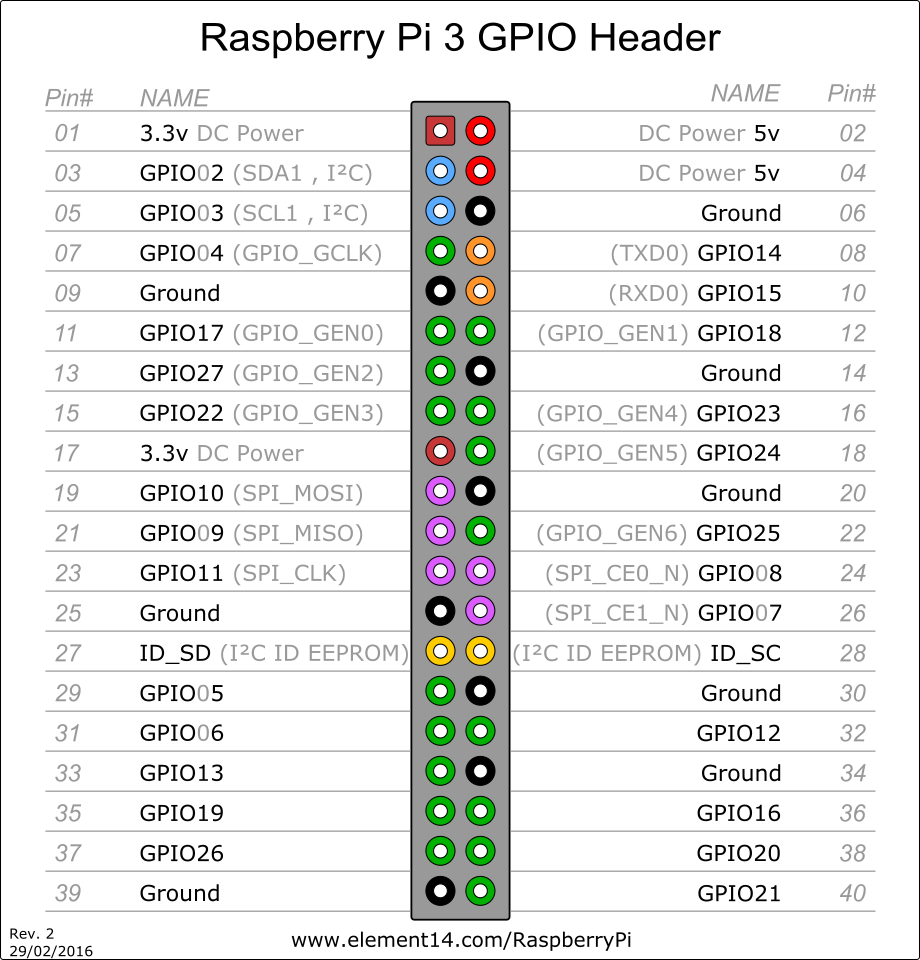
\includegraphics[width=\columnwidth]{rasp.eps}
\caption{Raspberry Pi Pin Configuration}
\label{rasp}
\end{figure}

\begin{table}[!h]
\centering
\resizebox{0.52\columnwidth}{!}{%
\begin{tabular}{|c|c|}
\hline
\textbf{Raspberry Pi} & \textbf{STM32} \\ \hline
GND (Pin 6)           & GND            \\ \hline
3.3V (Pin 1)          & 3.3V           \\ \hline
GPIO 24               & SWDIO           \\ \hline
GPIO 25               & SCLK           \\ \hline
GPIO 18               & RESET          \\ \hline
\end{tabular}%
}
\caption{Raspberry Pi and STM32 Connections}
\label{raspstm}
\end{table}
The hardware connections between STM32 and the breadboard are available in Table \ref{stm32}.
\begin{table}[htbp]
\centering
\resizebox{0.5\columnwidth}{!}{%
\begin{tabular}{|c|c|}
\hline
\textbf{STM32 Pins} & \textbf{LED}       \\ \hline
PC13                & +ve                \\ \hline
GND                 & -ve (via resistor) \\ \hline
\end{tabular}%
}
\caption{STM32 and LED connection}
\label{stm32}
\end{table}

\begin{figure}[thpb]
\centering
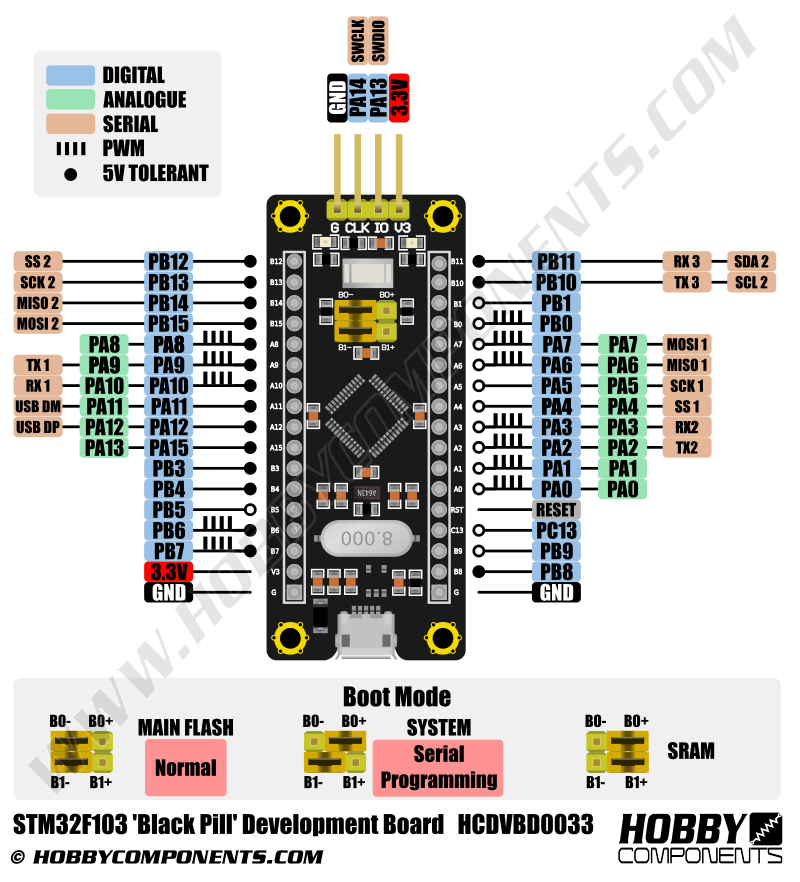
\includegraphics[width=\columnwidth]{stm.eps}
\caption{STM32f103c8t6 Pin Configuration}
\label{stm32}
\end{figure}

\section{Software Setup}
\subsection{Installation and Configuration of OpenOCD}
\begin{lstlisting}[frame=single, breaklines]
sudo apt-get install git autoconf libtool make pkg-config libusb-1.0-0 libusb-1.0-0-dev

sudo apt install gcc-arm-none-eabi

git clone git://git.code.sf.net/p/openocd/code openocd-code

cd openocd-code

./bootstrap

./configure --enable-sysfsgpio --enable-bcm2835gpio

make

sudo make install
\end{lstlisting}

\section{Make File and Flashing}
\begin{lstlisting}
cd ~
git clone https://github.com/alokkesari/STM32F103C8T6.git
cd STM32F103C8T6
sudo make flash
\end{lstlisting}
%\subsection{Boot-loader Configuration}
%\begin{lstlisting}[frame=single, breaklines]
%cd ~
%
%mkdir jtag
%
%cd jtag
%
%nano openocd.cfg
%\end{lstlisting}
%Download the files from the following git repository:
%\begin{lstlisting}[frame=single, breaklines]
%https://github.com/ubogdan/STM32F103C8T6/blob/master/bootloader/generic_boot20_pc13.bin
%\end{lstlisting}
%Type the following commands in the jtag/openocd.cfg file and save.
%\begin{lstlisting}[language=bash, frame=single, breaklines]
%source [find interface/raspberrypi2-native.cfg]
%
%transport select swd
% 
%source [find target/stm32f1x.cfg]
%
%reset_config srst_only
%
%reset_config  srst_nogate
%
%reset_config srst_open_drain
% 
%adapter_nsrst_delay 100
%
%adapter_nsrst_assert_width 100
%
%\end{lstlisting}
%\subsection{Binary File Generation and Flashing the Micro-controller using Makefile}
%For generating binary file from the Embedded C code, download the Makefile for the corresponding STM32 micro-controller being used, in the bootloader folder, and run:
\textbf{Note:} Reset push button on the STM32 micro-controller needs to be pressed multiple times before flashing.
%\begin{lstlisting}[language=bash, frame=single, breaklines]
%sudo make flash
%\end{lstlisting}
\end{document}
